
{
    {
        \begin{figure}
             \centering
             \begin{subfigure}{\textwidth}
                 \centering
                 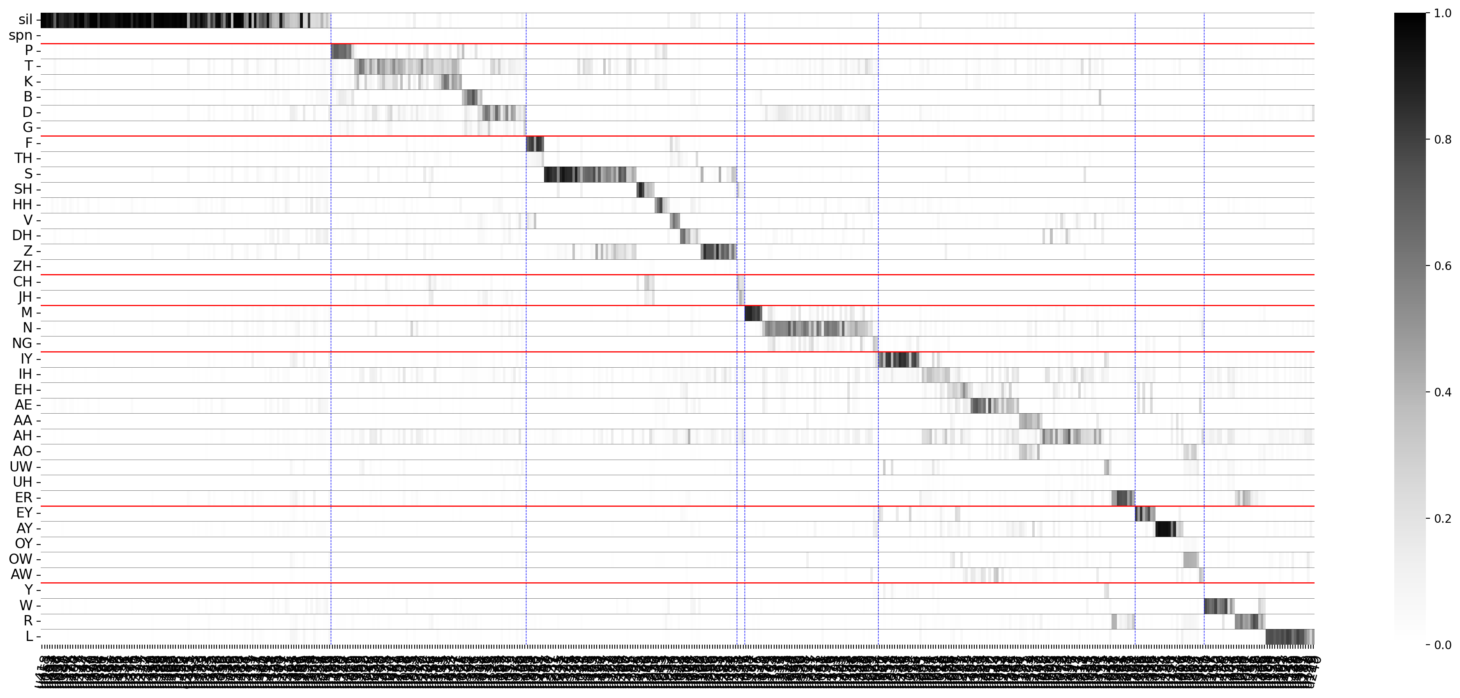
\includegraphics[width=1\linewidth]{figures/ch4figs/hub-u050-ap0500-givenunit-byphn.png}
                 \caption{分群數 50}
                 \label{fig:hub-u050-ap0500-givenunit-byphn--picked}
             \end{subfigure}
             \vfill
             \begin{subfigure}{\textwidth}
                 \centering
                 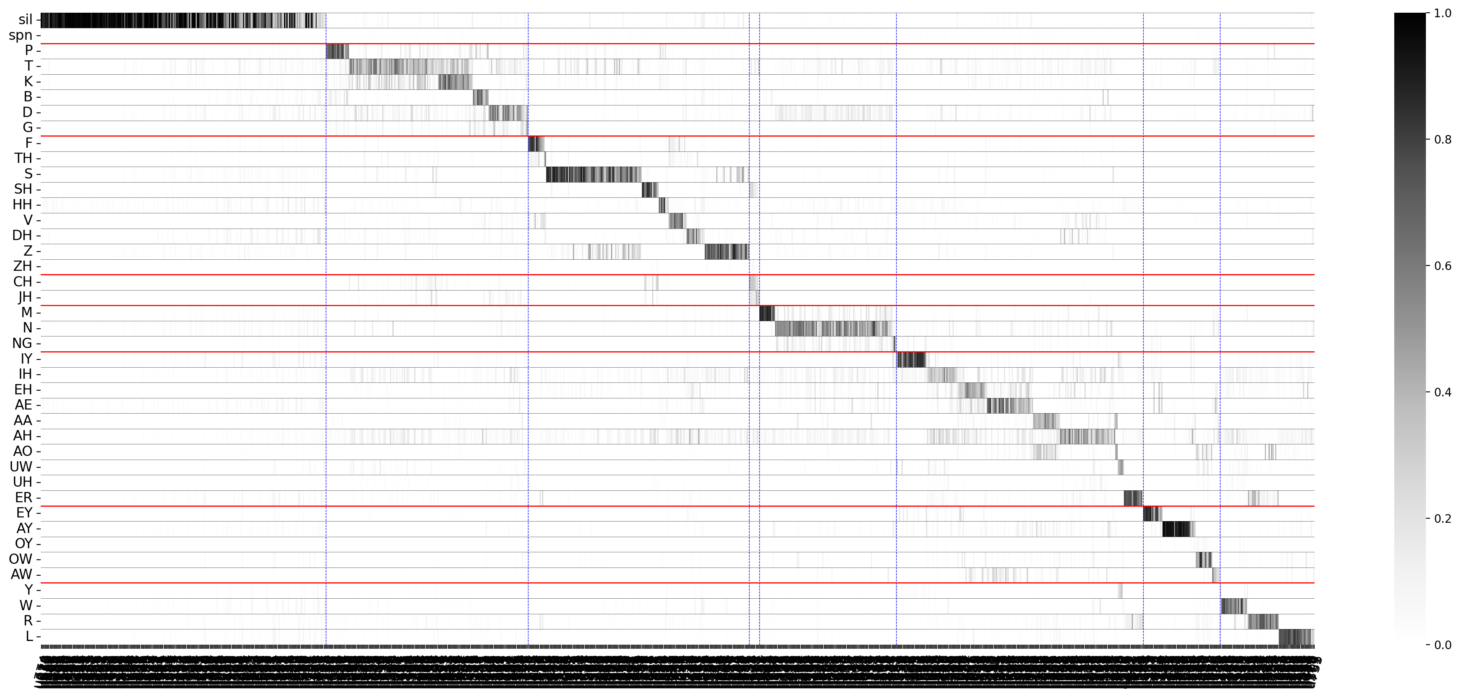
\includegraphics[width=1\linewidth]{figures/ch4figs/hub-u050-ap1000-givenunit-byphn.png}
                 \caption{分群數 100}
                 \label{fig:hub-u100-ap0500-givenunit-byphn--picked}
             \end{subfigure}
             \caption{比較同樣 500 種次詞單位的聲學片段模型,著重比較 HuBERT 表徵}
             在 K-平均演算法使用分群數 50 與 100 的條件機率熱圖 $p_{y|z}(i|j)$ 差異
             \label{fig:check-ap0500}
        \end{figure}
    }
}
